\documentclass[tikz]{standalone}

\usepackage{pgfplots}
\pgfplotsset{width=10cm, compat=1.18}


\begin{document}
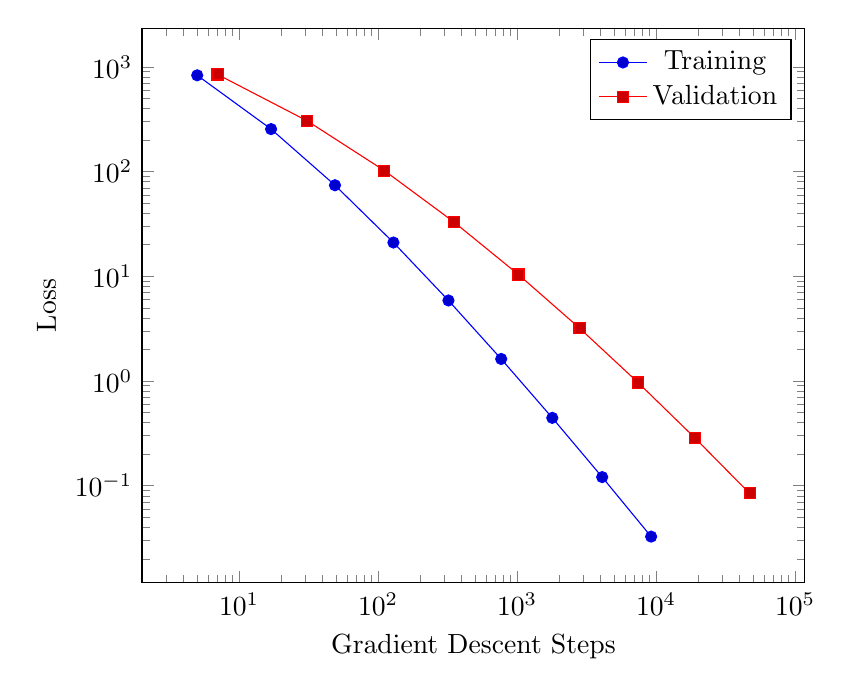
\begin{tikzpicture}
\begin{loglogaxis}[xlabel=Gradient Descent Steps,ylabel=Loss]
\addplot coordinates {
(5, 8.31160034e+02)
(17, 2.54685628e+02)
(49, 7.40715288e+01)
(129, 2.10192154e+01)
(321, 5.87352989e+00)
(769, 1.62269942e+00)
(1793, 4.44248889e-01)
(4097, 1.20714122e-01)
(9217, 3.26101452e-02)
};
\addplot coordinates {
(7, 8.47178381e+02)
(31, 3.04409349e+02)
(111, 1.02214539e+02)
(351, 3.30346265e+01)
(1023, 1.03886535e+01)
(2815, 3.19646457e+00)
(7423, 9.65789766e-01)
(18943, 2.87339125e-01)
(47103, 8.43749881e-02)
};
\legend{Training,Validation}
\end{loglogaxis}
\end{tikzpicture}
\end{document}
